\documentclass[a4paper,12pt,times,print,index, custombib]{PhDThesisPSnPDF}\usepackage[]{graphicx}\usepackage[]{color}
%% maxwidth is the original width if it is less than linewidth
%% otherwise use linewidth (to make sure the graphics do not exceed the margin)
\makeatletter
\def\maxwidth{ %
  \ifdim\Gin@nat@width>\linewidth
    \linewidth
  \else
    \Gin@nat@width
  \fi
}
\makeatother

\definecolor{fgcolor}{rgb}{0.345, 0.345, 0.345}
\newcommand{\hlnum}[1]{\textcolor[rgb]{0.686,0.059,0.569}{#1}}%
\newcommand{\hlstr}[1]{\textcolor[rgb]{0.192,0.494,0.8}{#1}}%
\newcommand{\hlcom}[1]{\textcolor[rgb]{0.678,0.584,0.686}{\textit{#1}}}%
\newcommand{\hlopt}[1]{\textcolor[rgb]{0,0,0}{#1}}%
\newcommand{\hlstd}[1]{\textcolor[rgb]{0.345,0.345,0.345}{#1}}%
\newcommand{\hlkwa}[1]{\textcolor[rgb]{0.161,0.373,0.58}{\textbf{#1}}}%
\newcommand{\hlkwb}[1]{\textcolor[rgb]{0.69,0.353,0.396}{#1}}%
\newcommand{\hlkwc}[1]{\textcolor[rgb]{0.333,0.667,0.333}{#1}}%
\newcommand{\hlkwd}[1]{\textcolor[rgb]{0.737,0.353,0.396}{\textbf{#1}}}%

\usepackage{framed}
\makeatletter
\newenvironment{kframe}{%
 \def\at@end@of@kframe{}%
 \ifinner\ifhmode%
  \def\at@end@of@kframe{\end{minipage}}%
  \begin{minipage}{\columnwidth}%
 \fi\fi%
 \def\FrameCommand##1{\hskip\@totalleftmargin \hskip-\fboxsep
 \colorbox{shadecolor}{##1}\hskip-\fboxsep
     % There is no \\@totalrightmargin, so:
     \hskip-\linewidth \hskip-\@totalleftmargin \hskip\columnwidth}%
 \MakeFramed {\advance\hsize-\width
   \@totalleftmargin\z@ \linewidth\hsize
   \@setminipage}}%
 {\par\unskip\endMakeFramed%
 \at@end@of@kframe}
\makeatother

\definecolor{shadecolor}{rgb}{.97, .97, .97}
\definecolor{messagecolor}{rgb}{0, 0, 0}
\definecolor{warningcolor}{rgb}{1, 0, 1}
\definecolor{errorcolor}{rgb}{1, 0, 0}
\newenvironment{knitrout}{}{} % an empty environment to be redefined in TeX

\usepackage{alltt}
%\documentclass[a4paper,12pt,times,numbered,print,index]{PhDThesisPSnPDF}

\usepackage{import}

\input{../Preamble/preamble}

%******************************** Glossary *********************************************
\usepackage[toc,acronym]{glossaries}
% suppress page number list in glossary:
%\usepackage[nonumberlist]{glossaries}

\makeglossaries

\renewcommand*{\glstextformat}[1]{\textsf{#1}}
%\renewcommand*{\glshyperlink}[1]{\textsf{#1}}

%--------------
% Glossary
%--------------
\newglossaryentry{fragment}{name=fragment, description={not a PCR duplicate. With paired reads from standard RAD (i. e. including random shearing of restriction fragments) typically identified by having different PE read sequences or different insert sizes after read mapping against a reference}}
\newglossaryentry{RAD tag}{name=RAD tag, description={genetic marker from RAD sequencing; the sequence up or downstream of a restriction site}}
\newglossaryentry{barcode}{name=barcode, description={short DNA sequence incorporated into adapter oligonucleotides that becomes part of the sequence read. Barcodes are used in order to be able to pool the DNA of different individuals, populations, treatments, etc. into one library that can be sequenced on one lane of an illumina flow cell}}
\newglossaryentry{index}{name=index, description={similar to barcode and serves the same purpose; generally incorporated into the centre of the adapter so that special sequencing run for the index is required} }
%\newglossaryentry{SbfI}{name=SbfI, description={restriction enzyme with the recognition sequence \includegraphics[scale=.5]{Sbf-I-cutsite_1_v1_000015}} }
\newglossaryentry{SbfI}{name=SbfI, description={restriction enzyme with the recognition sequence CCTGCA$\downarrow$GG} }
\newglossaryentry{XhoI}{name=XhoI, description={restriction enzyme with the recognition sequence C$\downarrow$TCGAG} }
\newglossaryentry{heterochromatin}{name=heterochromatin, description={Chromatin that remains in a highly condensed state throughout the cell cycle}}
\newglossaryentry{contig}{name=contig, description={longer consensus sequence derived from assembling smaller overlapping sequence reads}}
\newglossaryentry{linked RAD tag site}{name=linked RAD tag site, description={position in the reference sequence with at least one "properly mapped" read pair on either side of a putative restriction site and the SE reads overlapping each other as expected from the restriction enzyme}}
\newglossaryentry{proper pair}{name=proper pair, description={read pair from illumina paired-end sequencing that got mapped to a reference in the correct orientation within a maximum expected distance from each other that is determined by the fragment size selection during the sequencing library preparation}}
\newglossaryentry{kmer}{name=kmer, description={subsequence with a specified length (k) of a longer sequence}}
\newglossaryentry{e-value}{name=Expect (E) value, description={The Expect value (E) is a parameter that describes the number of hits one can "expect" to see by chance when searching a database of a particular size}}
\newglossaryentry{read}{name=read, description={any sequence that comes out of the sequencer}}
\newglossaryentry{edit distance}{name=edit distance, description={minimum number of operations (one symbol insertion, deletion or substitution) required to change one string of symbols into another. Also known as \emph{Levenshtein distance}}}
\newglossaryentry{Ct}{name={C$_{t}$}, description={PCR cycle when a certain fluorescent threshold is reached}}
\newglossaryentry{mqs}{name={mapping quality score}, description={The mapping quality score \emph{Q} is the Phred transformation of the estimate of the probability \emph{p} that the reported mapping position does not correspond to the read's true point of origin: $Q = -10 \log_{10} p$. The way \emph{p} is estimated is different for each mapping programme, but in any case a mapping quality score \emph{Q} of 3 roughly corresponds to a mis-mapping probability \emph{p} of 0.5, i. e. the read has an estimated 50\% chance to have derived from a location other than the one reported}}
\newglossaryentry{discordant}{name=discordant, description={A read pair that aligns with the expected relative mate orientation and with the expected range of distances between mates is said to align "concordantly". This is also called a \gls{proper pair}. If both mates have unique alignments, but the alignments do not match paired-end expectations (i.e. the mates aren't in the expected relative orientation, or aren't within the expected distance range, or both), the pair is said to align "discordantly"}}

%----------------
% Acronyms
%----------------
\newacronym{snp}{SNP}{single nucleotide polymorphism}
\newacronym{rad}{RAD}{Restriction Site associated DNA}
\newacronym{pe}{PE}{paired-end}
\newacronym{se}{SE}{single-end}
\newacronym{bp}{bp}{base pair}
\newacronym{indel}{indel}{sequence insertion or deletion polymorphism}
\newacronym{SAM}{SAM}{Sequence Alignment/Map format}
\newacronym{EST}{EST}{expressed sequence tag}

%%%%%% -- KNITR SETUP -- %%%%%%%%%%

%%%%%%%%%%%%%%%%%%%%%%%%%%
\IfFileExists{upquote.sty}{\usepackage{upquote}}{}
\begin{document}

\tableofcontents

\listoffigures

\listof{cmd}{List of commands}

\printglossaries

\chapter{Testing incomplete digestion}

% **************************** Define Graphics Path **************************
\ifpdf
    \graphicspath{
    {./Figs/Raster/}
    {./Figs/PDF/}
    {./Figs/}
    }
\else
    \graphicspath{ 
    {./Figs/Vector/}
    {./Figs/}
%    {/Users/Claudius/Documents/PhD/THESIS/kks32/LaTeX/3_Chapter/Figs}
    }
\fi


% ************************************************************************************

%\epigraph{Nothing in biology makes sense, except in the light of evolution}{Theodosius Dobzhansky}
%
%\epigraph{\dots it occurred to me to ask the question, Why do some die and some live? And the answer was clearly, that on the whole the best fitted live. [\dots] Then it suddenly flashed upon me that this self-acting process would necessarily improve the race, because in every generation the inferior would inevitably be killed off and the superior would remain-that is, the fittest would survive \dots}{Alfred Russel Wallace}

\epigraph{
Bonzai: Are you as successful as you would like to be?

Zappa: I would say that the basic characteristic of my life is failure. 
If there is one thing that I excel at, it's failure -- I manage to fail at 100 percent of the things that I do. 
Since most of the things that I set out to do are theoretically impossible, it's very easy to fail. 
I've learned to live with it. 
In terms of machinery and personnel, there never seems to be enough to get things done exactly right.
}{interview with Frank Zappa, 1985}

% ------------------------------------------------------------------------------------------------

% ------------------------------------------------------------------------------------------------

% --------------------------------
\section{Introduction}
% --------------------------------
The initial goal was to do a hybrid zone analysis and a QTL mapping study with a genetic marker technique that would allow the reliable scoring of genotypes at 1000$+$ loci in the genome of the grasshoppers at relatively low cost. The \gls{rad} marker technique, first described by \cite{Baird2008}, seemed to fulfil that promise.

%% ------------------------------------
\subsection{Why use RAD?}
%% ------------------------------------
\gls{rad}, aka RADseq, is the high-throughput sequencing of restriction fragment ends (figure \ref{RAD_protocol_overview}). It requires no prior genome sequence information. Only genome size and GC content are required to estimate the required number of reads for a certain target coverage. 
RADseq can yield co-dominant \gls{snp} markers in \glspl{RAD tag}, dominant presence/absence markers when the restriction site sequence is polymorphic or short indel polymorphisms when the clustering algorithm allows for them. Additionally, when doing \gls{pe} sequencing, a \gls{pe} contig can be assembled for a given \gls{RAD tag} (figure \ref{RAD_protocol_overview}).
Given enough coverage and when using adapters with barcode sequences, individual genotypes can be scored which is required for hybrid zone analysis (especially genomic clines analysis) as well as QTL mapping. 

Since the original version of \gls{rad} sequences tags around every restriction site (figure \ref{RAD_protocol_overview}), it allows for only limited complexity reduction. Further complexity reduction can be achieved by skipping the step of shearing the restriction fragments and instead size selecting a range of restriction fragments that have the right size for the sequencing platform. Further fine tuning of fragment number can be achieved when digesting DNA with two enzymes, so-called double-digest \gls{rad} (figure \ref{ddRAD_protocol_overview}) \citep{Peterson2012}.
% ---- add glossary entrywithout generating text ----
\glsadd[]{barcode} % allows to use \glshyperlink in captions

\begin{figure}
\centering
\includegraphics[width=.7\textwidth]{RADprotocolOverview}
\caption[Overview of the RAD marker technique.]{Overview of the \gls{rad} marker technique. (1) One restriction enzyme is used to digest genomic DNA. The first illumina adapter (P1), containing a different \glshyperlink[\textsf{barcode}]{barcode} (here called \gls{index}) sequence for each individual, is then ligated to the restriction fragments. The restriction fragments are then sheared, usually by high-frequency sonication, into a fragment size range that is suitable for illumina sequencing, which is selected on an agarose gel. After ligation of the second illumina adapter (P2), fragments with at least one P1 adapter are enriched by selective PCR. (2) The \gls{se} reads start with a barcode sequence, followed by the remainder of the restriction site. Only relatively short sequences (tags) are generated from the ends of the fragments. (3) Due to random shearing of restriction fragments, the \gls{pe} reads start at variable genomic distance from the restriction site (unless they are PCR duplicates) and thus can be assembled into short \gls{pe} contigs, depending on the size range selected on the gel. Taken from \cite{Atwood2011}. }
\label{RAD_protocol_overview}
\end{figure}

\begin{figure}
%\includegraphics[width=\textwidth]{/Users/Claudius/Documents/PhD/sRAD/RAD_sketches/RAD_sketches}\\
%\includegraphics[width=\textwidth]{/Users/Claudius/Documents/PhD/sRAD/RAD_sketches/RAD_sketches_1}\\
\def\svgwidth{.9\textwidth}
\subimport{./Figs/Inkscape_Graphics/}{ddRAD_overview_1.pdf_tex}\\ 
\def\svgwidth{\textwidth}
\subimport{./Figs/Inkscape_Graphics/}{ddRAD_overview_2.pdf_tex}\\
\def\svgwidth{.9\textwidth}
\subimport{./Figs/Inkscape_Graphics/}{ddRAD_overview_3.pdf_tex}\\
\def\svgwidth{.9\textwidth}
\subimport{./Figs/Inkscape_Graphics/}{ddRAD_overview_4.pdf_tex}\\
\def\svgwidth{.9\textwidth}
\subimport{./Figs/Inkscape_Graphics/}{ddRAD_overview_5.pdf_tex}
\caption[Double-digest RAD protocol overview.]{Double-digest RAD protocol overview.}
\label{ddRAD_protocol_overview}
\end{figure}

\begin{figure}[t]
\ContinuedFloat
\caption[]{Genomic DNA is first digested by two different restriction enzymes (red and green). Illumina adapters (P1 and P2) are then ligated to the restriction fragments. The P2 adapter is a so-called divergent-Y adapter that only contains the reverse-complement of the backward PCR primer binding site needed during the selective PCR step. Restriction fragments are then size-selected on a gel. Here, in contrast to the standard RAD protocol (see fig. \ref{RAD_protocol_overview}), gel size selection selects which markers get into the final sequencing library. The selective PCR step enriches the library for fragments with at least one P1 adapter ligated to it. Bridge-amplification on the illumina flow cell requires a P1 and a P2 adapter. Illumina paired-end sequencing results in two RAD tags per fragment that can be assembled and used for SNP and indel calling.}
\end{figure}


%% ------------------------------------
\subsection{The Problem}
%% ------------------------------------

A standard RAD was prepared according to the protocol of Paul Etter, (University of Oregon, \citealt{Baird2008}). The RAD library contained DNA from 36 grasshoppers sampled from the two distal populations ("Aunat" and "Greixer") of a transect through the \textit{Chorthippus parallelus / erythropus} hybrid zone in the Pyrenees between France and Spain. The RAD library was sequenced on an illumina GAIIx and the resulting reads assembled with the programme suite \texttt{stacks} \citep{Catchen2011}.

Figure \ref{Big_Data:freq_dist_of_genotype_calls} shows the frequency distribution of loci -- reconstructed by \texttt{stacks} version 0.998 -- over the number of individuals that have a genotype called for that locus. \texttt{Stacks} was run with a minimum allele coverage of 3 per individual and a maximum number of mismatches between alleles of 2 for merging alleles into loci within individuals as well as assembling a catalog of loci for the whole sample of 36 grasshoppers (further details can be looked up on the \href{http://creskolab.uoregon.edu/stacks/param_tut.php}{\texttt{stacks}} home page). About 50\% of the 379,720 unfiltered reconstructed loci have only a genotype call in one or two of the 36 individuals. About 170,000 RAD markers were expected from this library (see section \ref{ch:RAD_marker_number}) assuming a genome size of 12 giga \glspl{bp} (see section \ref{ch:Genome_size}).

%\begin{figure}
%\centering
%<<freq dist of genotype calls Big Data, echo=FALSE, out.width='.9\\linewidth', cache=TRUE>>=
%@
%\caption{Frequency distribution of loci, reconstructed by \texttt{stacks} (i. e. so-called "catalog stacks"), over the number of individuals in which they have a genotype call.}
%\label{Big_Data:freq_dist_of_genotype_calls}
%\end{figure}

Figure \ref{ddRAD:freq_dist_of_genotype_calls} shows the frequency distribution of reconstructed loci over the number of individuals for which they have a genotype called for the data of an \gls{SbfI}$+$\gls{XhoI} double-digest RAD library. The \gls{se} and \gls{pe} \glspl{RAD tag} have been merged before the assembly with \texttt{stacks}. \texttt{Stacks} was run with a minimum allele depth of 3 and maximum mismatch distance of 6 for merging alleles into read stacks within individuals as well as assembling a catalog stack from the individual stacks of all 36 grasshoppers (plus 2 technical replicates). Of the 156,532 loci (i. e. catalog stacks) that \texttt{stacks} had assembled, 51\% can only be found in one individual and only 3.5\% can be found in 20 or more individuals. Around 16,000 RAD markers were expected from this double-digest library (see equation \ref{eq:exp_number_ddRAD_loci} in chapter \ref{ch:RAD_marker_number}).

%\begin{figure}
%\centering
%<<freq dist of genotype calls SbfI-XhoI, echo=FALSE, out.width='.9\\linewidth', cache=TRUE>>=
%@
%\caption{Frequency distribution of catalog tags over the number of individuals in which they have a genotype call.}
%\label{ddRAD:freq_dist_of_genotype_calls}
%\end{figure}

\begin{figure}
\centering
\begin{subfigure}[t]{.495\textwidth}
\begin{knitrout}
\definecolor{shadecolor}{rgb}{0.969, 0.969, 0.969}\color{fgcolor}

{\centering \includegraphics[width=.9\linewidth]{figure/freq_dist_of_genotype_calls_Big_Data-1} 

}



\end{knitrout}
\caption{}
\label{Big_Data:freq_dist_of_genotype_calls}
\end{subfigure}
\hfill
\begin{subfigure}[t]{.495\textwidth}
\begin{knitrout}
\definecolor{shadecolor}{rgb}{0.969, 0.969, 0.969}\color{fgcolor}

{\centering \includegraphics[width=.9\linewidth]{figure/freq_dist_of_genotype_calls_SbfI-XhoI-1} 

}



\end{knitrout}
\caption{}
\label{ddRAD:freq_dist_of_genotype_calls}
\end{subfigure}
\caption{Frequency distribution of loci, reconstructed by \texttt{stacks} (i. e. so-called "catalog stacks"), over the number of individuals in which they have a genotype call.}
\end{figure}



\begin{enumerate}
\item describe observation of SbfI sites in RAD reads
\item incomplete digestion as a possible underlying cause
%\item assembly/clustering of reads into putative RAD tags
\end{enumerate}


%% ---------------------------------------------------
\section{Methods \& and Results}
%% ---------------------------------------------------

\begin{itemize}
\item work off questions
\item leave details including command lines for suppl. material
\item template amount estimation with fluorometer before and after PCR, qPCR
\item how much heterozygosity within populations, after long distance dispersal
\item leap-frog dispersal
\item Lunt, Cooper, Cpn1, mitochondria
\end{itemize}

%% ---------------------------------------------------
\section{Supplementary Methods}
%% ---------------------------------------------------

%% ---------------------------------------------------
\section{Adapter sequences for SbfI$+$XhoI ddRAD}
%% ---------------------------------------------------
\begin{figure}[h]
\begin{Verbatim}[fontfamily=courier, fontsize=\relsize{-7}, commandchars=\\\{\}, frame=single, framesep=10pt, label=P1 and P2 adapters for ddRAD]
          {\footnotesize P1 adapter}                                        {\footnotesize insert}                                   {\footnotesize P2 adapter}
5'-\underline{AATGATACGGCGACCACCGA}GATCTACACTCTTTCCCTACACGA\colorbox{white}{CGCTCTTCCGATCT}xxxxx{\color{blue}TGC*A}     GGNNNNNNNNNNNC     P-{\color{red}TCGA}\colorbox{orange}{A-GATCGGAAGAGCG}GTTCAGCAGGAATGCCGAGACCG\rotatebox{30}{\textit{TAGAGCATA*C}-3'}
3'-TTACTATGCCGCTGGTGGCTCTAGATGTGAGAAAGGGATGTGCT\colorbox{orange}{GCGAGAAGGCTAGA}xxxxx-P    {\color{blue}ACGT}CCNNNNNNNNNNNG{\color{red}AGCT}       \colorbox{white}{T*CTAGCCTTCTCGC}CAAGTCGTCCTTACGGCTCTGGCTAG\underline{AGCATACGGCAGAAGACGAAC-5'}
\end{Verbatim}
\caption{Outline of P1 and P2 adapters for double-digest RAD. Underlined sequences are selective PCR primer sequences. An asterisk * stands for a phosphorothioate bond. A "P" stands for a phosphate group. Sequences in \textit{italics} are non-complementary (wavy). Sequences with an orange background are identical to each other. An "x" stands for a base in a barcode sequence.}
\label{adapter-outline} % note, label has to come after caption
\end{figure}


%% ---------------------------------------------------
\FloatBarrier
\subsection{Estimating genome wide GC content}\label{ch:gc}
%% ---------------------------------------------------

\begin{cmd}
\begin{Verbatim}[formatcom=\color{darkgray}, fontsize=\scriptsize]

$ for i in *fq_2.gz; do ( awk '(NR-2)%4==0' <(zcat $i) | perl -ne' $h{$_}=1;END{foreach $s (keys %h)
{$gc += $s =~ tr/GC/GC/;} print $gc/(51 * scalar keys %h), "\n";} ' )& done | 
perl -ne'$sum+=$_; END{print $sum/$., "\n";}'

0.4607
\end{Verbatim}
\caption[Determine GC content from standard RAD PE reads]{For each individual, this command takes the \glspl{pe} reads, uniques them and determines their overall GC content. Finally, the average of the individual GC contents is taken. Note the brute-force parallelisation by sending each iteration of the \texttt{for} loop into the background with \texttt{(\ldots )\&}.}
\label{cmd:GC_1}
\end{cmd}

Using the \gls{se} reads from the \gls{SbfI} RAD library (excluding the SbfI recognition sequence part) and command \ref{cmd:GC_2} I have determined the GC content of the \gls{se} reads: 49.5\%.

\begin{cmd}
\begin{Verbatim*}[formatcom=\color{darkgray}, fontsize=\scriptsize, numbers=left]
$ gc(){ awk '(NR-2)%4==0' | sed 's/^......//' |
perl -ne'$h{$_}=1;END{foreach $s (keys %h){$gc+=$s=~tr/GC/GC/;} print $gc/(40*scalar keys %h), "\n";}' ;}
$ export -f gc
$ mean(){ perl -ne'$sum+=$_; END{print $sum/$., "\n";}'; }
$ export -f mean
$ parallel -j 10 'zcat {} | gc' ::: *fq_1.gz | mean

0.4956
\end{Verbatim*}
\caption[Determine GC content of \gls{se} reads]{This command is a different version of command \ref{cmd:GC_1}. However, it is used here to determine the GC content of all \gls{se} reads from the standard \gls{SbfI} RAD library. It first creates and exports two functions, \texttt{gc} and \texttt{mean}, and then uses the programme \texttt{parallel} in order to parallelise the determination of GC content over 10 cores. After stripping barcode and the remainder of the restriction site, the reads are 40 base pairs long. Note, the space between \{ and \texttt{awk} (line 1) as well as \{ and \texttt{perl} (line 4) is required.}
\label{cmd:GC_2}
\end{cmd}

So, it seems that sequences close to \gls{SbfI} sites are more GC rich than further distant sequences. 

%% --------------------------------------------------------------------------------------------------------------------------
\FloatBarrier
\section{Genome size of \textit{Chorthippus parallelus}}\label{ch:Genome_size}
%% --------------------------------------------------------------------------------------------------------------------------

\textit{Chorthippus parallelus} has a chromosome complement of 2n = 16 + X. Males have one X-chromosomes, females have two. Table \ref{ta:genome_size_studies} shows four studies that provide genome size estimates for \textit{Chorthippus parallelus}. Note that all studies are measuring the DNA content of spermatids. However, none of the studies explicitly deal with the issue that half of their measurements are missing the contribution from the X chromosome. Table \ref{ta:genome_size_studies} mentions the country of origin of the grasshoppers used for genome size estimates. Note, however, that only \cite{Belda1991} provide sampling locations. For the rest it is assumed that individuals were sampled closed to the authors institutes. So two studies provide genome size estimates for \textit{C. parallelus parallelus} and two for \textit{C. parallelus erythropus}. The \textit{parallelus} subspecies seems to have a genome 2--4 giga \glspl{bp} larger than the one of subspecies \textit{erythropus}. Apart from possible systematic differences in methodology, this apparent difference in genome size could be real, since several studies have shown chromosomal differentiation between the two subspecies, in particular on the X chromosome: an active nucleolar organiser region (NOR) distally on the X in \textit{C. p. parallelus} but not in \textit{C. p. erythropus} \citep{Gosalvez1988}. This NOR on X lies in or near a distinctive distal C-band\footnote{\gls{heterochromatin} stained with Giemsa}. In addition, Pyrenean \textit{C. p. erythropus} also show an interstitial C-band on X that does not occur in pure \textit{C. p. parallelus} \citep{Bella2007}. Further chromosomal differences are listed in table 1 of \cite{Ferris1993}.

\ctable[
width=\textwidth,
doinside={ \relsize{-1.5} \setlength{\tabcolsep}{3pt} },
caption=Studies that provide genome size estimates for \textit{Chorthippus parallelus},
cap=Genome size estimates,
label=ta:genome_size_studies
]
{l c >{\raggedleft}p{.6cm}@{.}l >{\centering}p{2.5cm} l X}
{
\tnote[a]{\scriptsize see their table 3}
\tnote[b]{\scriptsize 5 individuals}
\tnote[c]{\scriptsize assuming 6.4 on relative scale corresponds to C-value of 5.5 pg}
\tnote[d]{\scriptsize see their table 2}
\tnote[e]{\scriptsize \textit{C. longicornis} syn. of \textit{C. parallelus}}
\tnote[f]{\scriptsize 3 individuals}
\tnote[g]{\scriptsize 3 individuals}
}
{
\toprule
\multirow{2}{*}{\textbf{study}} & \multirow{2}{1cm}{\textbf{sample source}}  & \multicolumn{2}{c}{\textbf{C-value}} & \multirow{2}{*}{\textbf{Method}} & \multirow{2}{*}{\textbf{tissue type}} & \multirow{2}{*}{\textbf{standard species}} \\
                                      &                                                              & \multicolumn{2}{c}{ [$10^{-12}$g]} &                                &                                                 &                                                           \\
\midrule
\cite{John1966}\tmark[a] & UK & 12&37 ($\pm$ 0.75)\tmark[b] & Feulgen staining, microdensitometry & spermatid & \textit{Locusta migratoria}\tmark[c] \\[0.7cm]
\cite{Wilmore1975}\tmark[d] & UK & 13&36 ($\pm$ 0.04) & Feulgen staining, microdensitometry & spermatid & mouse spermatid \\[0.7cm]
\cite{Gosalvez1980}\tmark[e] & Spain & 8&58 ($\pm$ 0.47)\tmark[f]   & Feulgen staining, microdensitometry & spermatid & \textit{Allium cepa}, root tissue \\[0.7cm]
\cite{Belda1991} & Spain & 10&73 ($\pm$ 0.97)\tmark[g]  & Feulgen staining, microdensitometry & spermatid & chick erythrocytes \\
\bottomrule
}

\cite{Gosalvez1988} showed that all the heterochromatin present in both subspecies is particularly rich in GC DNA base pairs.


%\begin{table}
%\caption{Studies that provide genome size estimates for \textit{Chorthippus parallelus}}
%\label{ta:genome_size}
%\centering
%\small
%\resizebox{\textwidth}{!}{
%\begin{tabular}[h]{c c >{\raggedleft}p{.6cm}@{.}l >{\centering}p{3cm} c c}
%\toprule
%\multirow{2}{*}{\textbf{study}} & \multirow{2}{1cm}{\textbf{sample source}}  & \multicolumn{2}{c}{\textbf{C-value}} & \multirow{2}{*}{\textbf{Method}} & \multirow{2}{*}{\textbf{tissue type}} & \multirow{2}{*}{\textbf{standard species}} \\
%                                      &                                                              & \multicolumn{2}{c}{ [$10^{-12}$g]} &                                &                                                 &                                                           \\
%\midrule
%\cite{John1966} & UK & 12&37 $\pm$ 0.75 & Feulgen staining, microdensitometry & spermatid & \textit{Locusta migratoria}\\[0.7cm]
%\cite{Wilmore1975} & UK & 13&36  & Feulgen staining, microdensitometry & spermatid & mouse spermatid \\[0.7cm]
%\cite{Gosalvez1980} & Spain & 8&58   & Feulgen staining, microdensitometry & spermatid & \textit{Allium cepa}, root tissue \\[0.7cm]
%\cite{Belda1991} & Spain & 10&73  & Feulgen staining, microdensitometry & spermatid & chick erythrocytes \\
%\bottomrule
%\end{tabular}
%}
%\end{table}


%% --------------------------------------------------------------------------------------------------------------------------
\FloatBarrier
\subsection{Expected RAD marker number}\label{ch:RAD_marker_number}
%% --------------------------------------------------------------------------------------------------------------------------

Using PE reads from the standard RAD library -- uniqued  per individual -- as a proxy for the whole genome, I estimate the GC content of the \textit{Chorthippus parallelus} genome to be around 46\% (\ref{ch:gc}). However, \cite{Wilmore1975} have determined the GC content of the \textit{C. p. parallelus} genome from thermal dissociation profiles (41.2\%) and sedimentation in CsCl and Cs$_{2}$SO$_{4}$ density gradients (41.7\% and 42.0\%)\footnote{see their table 1}. I think that \gls{pe} reads from SbfI standard RAD are still a biased sample towards GC rich regions of the genome due to the GC rich \gls{SbfI} recognition sequence. 
Assuming a genome size of 12 giga base pairs, the expected number of RAD tag loci from a standard RAD library with \gls{SbfI} in the grasshopper genome is $\sim$170,000 (equation \ref{eq:exp_num_standard_RAD_loci}). 

\scriptsize
\begin{align}
\text{expected number of \glspl{RAD tag}} &= \underbrace{12 \times 10^{9}}_{\text{genome size}} \times 
\underbrace{ \left( \frac{0.42}{2}\right)^{6} \times \left( \frac{(1-0.42)}{2} \right)^{2} }_{\text{SbfI site probability}} \times 
\underbrace{2}_{\text{tags per SbfI site}}
\label{eq:exp_num_standard_RAD_loci} \\[5pt] 
&= 173,110 \nonumber
\end{align}
\normalsize

The number (and identity) of markers in a double-digest RAD library depends very much on the size selection of restriction fragments. I selected fragments roughly between 300 and 800 \gls{bp} length. The P1 adapter is 63 bp long (excluding 4 bp overhang), the P2 adapter is 61 bp long (excluding 4 bp overhang). The \gls{SbfI} remainder after the cut is 6 \gls{bp} long and the \gls{XhoI} remainder is 5 \gls{bp} long. If \gls{XhoI} cuts a fragment at a distance less than about $300 - 63 - 61 -6 -5 = 165$ \gls{bp} away from the SbfI cut site, then this fragment would not be size selected because it would be shorter than the lower bound of size selection (in this example). The \gls{se} sequences (excluding the SbfI recognition sequence parts) have a mean GC content of 49.5\% (see command \ref{cmd:GC_2}). 
The following formula requires the GC content of sequences of length 168 \gls{bp} adjacent to SbfI sites. I will use the average of \gls{se} and \gls{pe} GC contents -- 48\% (see~chapter \ref{ch:gc}) -- for calculating the probability of an XhoI cut within the first 168bp after the SbfI restriction site. In the next 500 \gls{bp} then needs to be at least one \gls{XhoI} site to make the SbfI fragment a marker.
The expected number of RAD markers per genome with an SbfI-XhoI double-digest and a selected size range of 300--800bp is:


\scriptsize
%\begin{preview}
\begin{align} % use align instead of equation for multi-line long equations
\text{RAD markers per genome} &\simeq 12 \times 10^{9} 
	&&\text{(genome size in bp)}  \label{eq:exp_number_ddRAD_loci} \\[5pt]
&\times \left(\frac{0.42}{2}\right)^{6}\times \left(\frac{(1-0.42)}{2}\right)^{2} &&\text{(SbfI cut prob. per bp)} \notag \\[5pt]
&\times 2 
	&&\text{(each cut creates two potential RAD tags)} \notag \\[5pt]
&\times \left[1-\left(\frac{0.48}{2}\right)^{4} \times \left( \frac{(1-0.48)}{2}\right)^{2} \right]^{165} 
	&&\text{(prob. of no XhoI cut in the first 165 bp after SbfI site)} \notag \\[5pt]
&\times \left(1- \left[1-\left(\frac{0.46}{4}\right)^{2} \times \left( \frac{(1-0.46)}{4}\right)^{4} \right]^{500} \right) 
	&&\text{(prob. of at least one XhoI cut in the following 500bp)} \notag \\[5pt]
%&\quad \times \ 2 \tag{two markers per SbfI cut{\color{red}*}}  \\
&\simeq 16,000 \nonumber
\end{align}
%\end{preview}
\normalsize

I have created an Excel file called \texttt{ComplexityReduction.xls} that implements equation \ref{eq:exp_number_ddRAD_loci} and that allows easy modification of variables.

%% ---------------------------------------------------
\section{Estimating divergence time of the two subspecies}
%% ---------------------------------------------------

\begin{itemize}
\item ABS, simCoal
\item long dispersal tail --> potential for contact between distal populations
\item test gene flow <-> no gene flow model
\item filtering paralogs in highly repetitive genomes
\item large genome size $+$ genome size variation
\item clustering algorithms: DNAclust, CD-Hit, afcluster, ustacks, starcode, UNEAK
\end{itemize}


\section{Results}

\section{Interpretation of Results}



% ********************************************************
And now I begin my third chapter here \dots

\cite{Baird2008} were the first to publish about RAD. \SI{12,3}{\micro\metre}

Fig.~\vref{fragments-mapped-per-ind} shows the number of \glspl{fragment} mapped per individual.
I am trying to find \glspl{snp} among individuals of the sample.
% ********************************************************

\begin{figure}
\begin{knitrout}
\definecolor{shadecolor}{rgb}{0.969, 0.969, 0.969}\color{fgcolor}

{\centering \includegraphics[width=\linewidth]{figure/fragments_mapped_per_ind-1} 

}



\end{knitrout}
\caption{Distribution of RAD fragment numbers mapped to 4 primer3ready reference contigs. 
A "fragment" is a properly mapped read pair from an individual with a unique insert size. 
If two read pairs on a RAD site from an individual have the same insert size, they constitute only one fragment, i. e. one read pair is likely to be a PCR duplicate.}
\label{fragments-mapped-per-ind}
\end{figure}





\subsection{First subsection in the first section}
\dots and some more 

\subsection{Second subsection in the first section}
\dots and some more \dots

\subsubsection{First subsub section in the second subsection}
\dots and some more in the first subsub section otherwise it all looks the same
doesn't it? well we can add some text to it \dots

\subsection{Third subsection in the first section}
\dots and some more \dots

\subsubsection{First subsub section in the third subsection}
\dots and some more in the first subsub section otherwise it all looks the same
doesn't it? well we can add some text to it and some more and some more and
some more and some more and some more and some more and some more \dots

\subsubsection{Second subsub section in the third subsection}
\dots and some more in the first subsub section otherwise it all looks the same
doesn't it? well we can add some text to it \dots

\section{Second section of the third chapter}
and here I write more \dots

\section{The layout of formal tables}
This section has been modified from ``Publication quality tables in \LaTeX*''
 by Simon Fear.

The layout of a table has been established over centuries of experience and 
should only be altered in extraordinary circumstances. 

When formatting a table, remember two simple guidelines at all times:

\begin{enumerate}
  \item Never, ever use vertical rules (lines).
  \item Never use double rules.
\end{enumerate}

These guidelines may seem extreme but I have
never found a good argument in favour of breaking them. For
example, if you feel that the information in the left half of
a table is so different from that on the right that it needs
to be separated by a vertical line, then you should use two
tables instead. Not everyone follows the second guideline:

There are three further guidelines worth mentioning here as they
are generally not known outside the circle of professional
typesetters and subeditors:

\begin{enumerate}\setcounter{enumi}{2}
  \item Put the units in the column heading (not in the body of
          the table).
  \item Always precede a decimal point by a digit; thus 0.1
      {\em not} just .1.
  \item Do not use `ditto' signs or any other such convention to
      repeat a previous value. In many circumstances a blank
      will serve just as well. If it won't, then repeat the value.
\end{enumerate}

A frequently seen mistake is to use `\textbackslash begin\{center\}' \dots `\textbackslash end\{center\}' inside a figure or table environment. This center environment can cause additional vertical space. If you want to avoid that just use `\textbackslash centering'


\begin{table}
\caption{A badly formatted table}
\centering
\label{table:bad_table}
\begin{tabular}{|l|c|c|c|c|}
\hline 
& \multicolumn{2}{c}{Species I} & \multicolumn{2}{c|}{Species II} \\ 
\hline
Dental measurement  & mean & SD  & mean & SD  \\ \hline 
\hline
I1MD & 6.23 & 0.91 & 5.2  & 0.7  \\
\hline 
I1LL & 7.48 & 0.56 & 8.7  & 0.71 \\
\hline 
I2MD & 3.99 & 0.63 & 4.22 & 0.54 \\
\hline 
I2LL & 6.81 & 0.02 & 6.66 & 0.01 \\
\hline 
CMD & 13.47 & 0.09 & 10.55 & 0.05 \\
\hline 
CBL & 11.88 & 0.05 & 13.11 & 0.04\\ 
\hline 
\end{tabular}
\end{table}

\begin{table}
\caption{A nice looking table}
\centering
\label{table:nice_table}
\begin{tabular}{l c c c c}
\hline 
\multirow{2}{*}{Dental measurement} & \multicolumn{2}{c}{Species I} & \multicolumn{2}{c}{Species II} \\ 
\cline{2-5}
  & mean & SD  & mean & SD  \\ 
\hline
I1MD & 6.23 & 0.91 & 5.2  & 0.7  \\

I1LL & 7.48 & 0.56 & 8.7  & 0.71 \\

I2MD & 3.99 & 0.63 & 4.22 & 0.54 \\

I2LL & 6.81 & 0.02 & 6.66 & 0.01 \\

CMD & 13.47 & 0.09 & 10.55 & 0.05 \\

CBL & 11.88 & 0.05 & 13.11 & 0.04\\ 
\hline 
\end{tabular}
\end{table}


\begin{table}
\caption{Even better looking table using booktabs}
\centering
\label{table:good_table}
\begin{tabular}{l c c c c}
\toprule
\multirow{2}{*}{Dental measurement} & \multicolumn{2}{c}{Species I} & \multicolumn{2}{c}{Species II} \\ 
\cmidrule{2-5}
  & mean & SD  & mean & SD  \\ 
\midrule
I1MD & 6.23 & 0.91 & 5.2  & 0.7  \\

I1LL & 7.48 & 0.56 & 8.7  & 0.71 \\

I2MD & 3.99 & 0.63 & 4.22 & 0.54 \\

I2LL & 6.81 & 0.02 & 6.66 & 0.01 \\

CMD & 13.47 & 0.09 & 10.55 & 0.05 \\

CBL & 11.88 & 0.05 & 13.11 & 0.04\\ 
\bottomrule
\end{tabular}
\end{table}

%----------------------------
% Bibliography
%----------------------------

\bibliographystyle{elsarticle-harv}
\bibliography{/Users/Claudius/Documents/MyLiterature/Literature}

\end{document}
